\documentclass[tikz,border=3pt]{standalone}
\usepackage{newtxtext,newtxmath}
\usetikzlibrary{arrows.meta}
\definecolor{paperink}{HTML}{3F4852}
\definecolor{paperblue}{HTML}{2457C5}
\definecolor{paperred}{HTML}{C43B3B}
\definecolor{papergreen}{HTML}{2E8B57}
\definecolor{papergold}{HTML}{B97800}
\definecolor{papergray}{HTML}{F1F3F5}
\begin{document}
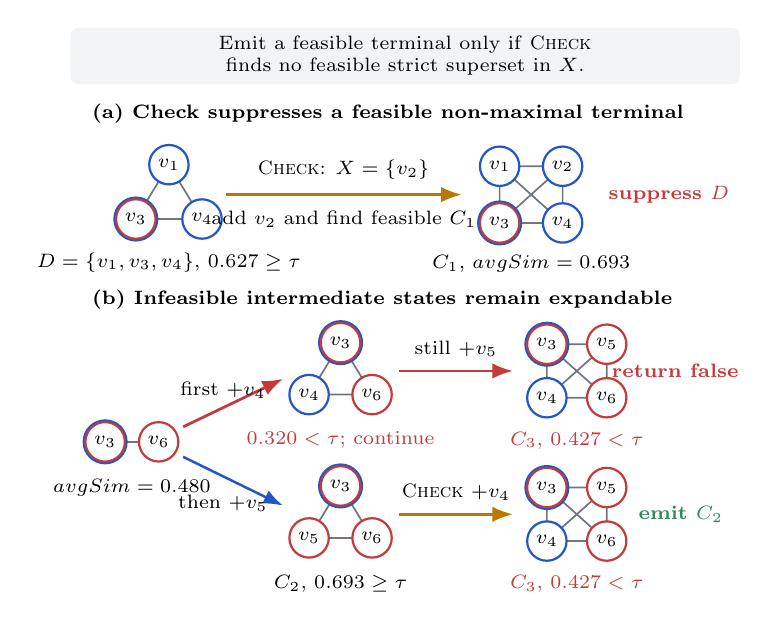
\begin{tikzpicture}[
  font=\scriptsize,
  >=Latex,
  vertex/.style={circle, draw=paperblue, fill=white, line width=0.8pt,
    minimum size=5.0mm, inner sep=0pt, font=\scriptsize},
  mone/.style={vertex, draw=paperblue},
  mtwo/.style={vertex, draw=paperred},
  vthree/.style={vertex, draw=paperred, line width=0.75pt,
    preaction={draw=paperblue, line width=2.05pt}},
  edge/.style={draw=paperink!75, line width=0.62pt},
  branch/.style={->, draw=paperblue, line width=0.9pt},
  checkarrow/.style={->, draw=papergold, line width=1.0pt},
  failarrow/.style={->, draw=paperred, line width=1.0pt},
  paneltitle/.style={font=\scriptsize\bfseries, anchor=west},
  note/.style={font=\scriptsize, align=center},
  rule/.style={draw=none, fill=papergray,
    minimum width=84mm, minimum height=7mm, align=center}
]

\fill[papergray, rounded corners=1mm]
  (-0.05,0.86) rectangle (8.45,1.58);
\node[font=\scriptsize, align=center, text width=82mm, inner sep=0pt]
  at (4.20,1.22)
  {Emit a feasible terminal only if \textsc{Check} finds no feasible strict superset in $X$.};

% Panel (a): CHECK suppresses an actual feasible non-maximal terminal.
\node[paneltitle] at (0.10,0.49) {(a) \textsc{Check} suppresses a feasible non-maximal terminal};

\begin{scope}[shift={(1.20,-0.54)}]
  \draw[edge] (0,0.38)--(-0.42,-0.31)--(0.42,-0.31)--cycle;
  \node[mone] at (0,0.38) {$v_1$};
  \node[vthree] at (-0.42,-0.31) {$v_3$};
  \node[mone] at ( 0.42,-0.31) {$v_4$};
  \node[note] at (0,-0.86) {$D=\{v_1,v_3,v_4\}$, $0.627\geq\tau$};
\end{scope}

\begin{scope}[shift={(5.80,-0.54)}]
  \coordinate (a) at (-0.40, 0.36);
  \coordinate (b) at (-0.40,-0.36);
  \coordinate (c) at ( 0.40, 0.36);
  \coordinate (d) at ( 0.40,-0.36);
  \draw[edge] (a)--(b)--(d)--(c)--cycle (a)--(d) (b)--(c);
  \node[mone] at (a) {$v_1$};
  \node[vthree] at (b) {$v_3$};
  \node[mone] at (c) {$v_2$};
  \node[mone] at (d) {$v_4$};
  \node[note] at (0,-0.88) {$C_1$, $\operatorname{avgSim}=0.693$};
\end{scope}
\draw[checkarrow] (1.92,-0.54)--(4.92,-0.54)
  node[midway,above=0.55mm,note] {\textsc{Check}: $X=\{v_2\}$}
  node[midway,below=0.75mm,note] {add $v_2$ and find feasible $C_1$};
\node[text=paperred, font=\scriptsize\bfseries] at (7.55,-0.54) {suppress $D$};

% Panel (b): an actual v6-owned branch showing infeasible continuation and backtracking.
\node[paneltitle] at (0.10,-1.88) {(b) Infeasible intermediate states remain expandable};

\begin{scope}[shift={(0.73,-3.68)}]
  \draw[edge] (-0.34,0)--(0.34,0);
  \node[vthree] at (-0.34,0) {$v_3$};
  \node[mtwo] at ( 0.34,0) {$v_6$};
  \node[note] at (0,-0.58) {$\operatorname{avgSim}=0.480$};
\end{scope}

% Upper branch: v4 is tried first; its infeasible state still expands by v5.
\begin{scope}[shift={(3.38,-2.78)}]
  \draw[edge] (0,0.36)--(-0.40,-0.30)--(0.40,-0.30)--cycle;
  \node[vthree] at (0,0.36) {$v_3$};
  \node[mone] at (-0.40,-0.30) {$v_4$};
  \node[mtwo] at (0.40,-0.30) {$v_6$};
  \node[note, text=paperred] at (0,-0.88) {$0.320<\tau$; continue};
\end{scope}
\draw[failarrow] (1.38,-3.49)--(2.65,-2.88)
  node[midway,above=0.4mm,note,xshift=-1.3mm,yshift=-1.2mm] {first $+v_4$};

\begin{scope}[shift={(6.38,-2.78)}]
  \coordinate (a) at (-0.38, 0.34);
  \coordinate (b) at (-0.38,-0.34);
  \coordinate (c) at ( 0.38, 0.34);
  \coordinate (d) at ( 0.38,-0.34);
  \draw[edge] (a)--(b)--(d)--(c)--cycle (a)--(d) (b)--(c);
  \node[vthree] at (a) {$v_3$};
  \node[mone] at (b) {$v_4$};
  \node[mtwo] at (c) {$v_5$};
  \node[mtwo] at (d) {$v_6$};
  \node[note, text=paperred] at (0,-0.88) {$C_3$, $0.427<\tau$};
\end{scope}
\draw[failarrow] (4.12,-2.78)--(5.57,-2.78)
  node[midway,above=0.45mm,note] {still $+v_5$};
\node[text=paperred, font=\scriptsize\bfseries] at (7.63,-2.78) {return false};

% Lower branch: after backtracking, v5 yields C2 and CHECK rejects C3.
\begin{scope}[shift={(3.38,-4.60)}]
  \draw[edge] (0,0.36)--(-0.40,-0.30)--(0.40,-0.30)--cycle;
  \node[vthree] at (0,0.36) {$v_3$};
  \node[mtwo] at (-0.40,-0.30) {$v_5$};
  \node[mtwo] at (0.40,-0.30) {$v_6$};
  \node[note] at (0,-0.88) {$C_2$, $0.693\geq\tau$};
\end{scope}
\draw[branch] (1.38,-3.87)--(2.65,-4.49)
  node[midway,below=0.4mm,note,xshift=-1.3mm] {then $+v_5$};

\begin{scope}[shift={(6.38,-4.60)}]
  \coordinate (a) at (-0.38, 0.34);
  \coordinate (b) at (-0.38,-0.34);
  \coordinate (c) at ( 0.38, 0.34);
  \coordinate (d) at ( 0.38,-0.34);
  \draw[edge] (a)--(b)--(d)--(c)--cycle (a)--(d) (b)--(c);
  \node[vthree] at (a) {$v_3$};
  \node[mone] at (b) {$v_4$};
  \node[mtwo] at (c) {$v_5$};
  \node[mtwo] at (d) {$v_6$};
  \node[note, text=paperred] at (0,-0.88) {$C_3$, $0.427<\tau$};
\end{scope}
\draw[checkarrow] (4.12,-4.60)--(5.57,-4.60)
  node[midway,above=0.45mm,note] {\textsc{Check} $+v_4$};
\node[text=papergreen, font=\scriptsize\bfseries] at (7.70,-4.60) {emit $C_2$};

\end{tikzpicture}
\end{document}
